% =============================================================
%  ONLINE RESOURCE 3 — Posterior Comparison: Laplace vs
%  Hamiltonian Monte Carlo
%  Supporting Information for Hackman & Zhu (2026)
%  "When Inverse Physics-Informed Neural Networks Become
%   Practically Identifiable: A Case Study in Synaptic Dopamine
%   Transport" — Medical & Biological Engineering & Computing
%   submission
% =============================================================
\documentclass[12pt]{article}

\usepackage[margin=1in]{geometry}
\usepackage[utf8]{inputenc}
\usepackage[T1]{fontenc}
\usepackage{lmodern}
\usepackage{amsmath, amssymb, mathtools}
\usepackage{graphicx}
\usepackage{booktabs}
\usepackage{hyperref}
\hypersetup{colorlinks=true, linkcolor=black, citecolor=black,
            urlcolor=blue, pdfborder={0 0 0}}
\usepackage{setspace}
\setlength{\parindent}{0pt}
\setlength{\parskip}{0.7em}

\title{Online Resource 3: Posterior Comparison --
Laplace vs Hamiltonian Monte Carlo \\
\large Supporting Information for ``When Inverse
Physics-Informed Neural Networks Become Practically
Identifiable: A Case Study in Synaptic Dopamine Transport''}

\author{Emmanuel Hackman and Huiqing Zhu \\
School of Mathematics and Natural Sciences, \\
University of Southern Mississippi, Hattiesburg, MS 39406, USA}

\date{}

\begin{document}
\maketitle

The Bayesian uncertainty quantification reported in the main text
(Results, \emph{Bayesian Uncertainty Quantification}) uses a Laplace
(Gaussian) approximation around the maximum a posteriori (MAP)
estimate of the analytical-model posterior. To validate the
Gaussian-approximation assumption, we independently drew $5{,}000$
samples from the same posterior using the No-U-Turn variant of
Hamiltonian Monte Carlo, implemented in Blackjax on the same GPU
device. The HMC chain used $1{,}000$ warm-up steps for
dual-averaging step-size and mass-matrix adaptation, followed by
$5{,}000$ post-warm-up samples; the log-posterior is the negative
Gaussian log-likelihood of the observation data under the
analytical 2D Gaussian forward model, scaled by
$1/(2\sigma_{\mathrm{noise}}^2)$ with
$\sigma_{\mathrm{noise}} = 0.02\,C_0$.

\begin{table}[h!]
\centering
\caption{\textbf{Posterior summary statistics: Laplace vs HMC.}
Both methods operate on the same $400$-observation dataset and the
same analytical-model likelihood. The two methods agree to three
decimal places in both posterior mean and standard deviation for $D$,
validating the Gaussian-approximation assumption of Laplace. Both
methods collapse to the lower boundary $k \to 0$ (see text), a model-
misspecification failure rather than a numerical artifact.}
\label{tab:hmc_vs_laplace}
\begin{tabular}{lcc}
\toprule
                       & \textbf{Laplace}        & \textbf{HMC}             \\
\midrule
$D$ posterior mean     & $0.3202$                & $0.3207$                 \\
$D$ posterior std      & $0.0114$                & $0.0114$                 \\
$D$ $95\%$ CI          & $[0.298,\ 0.343]$       & $[0.299,\ 0.344]$        \\
$k$ posterior mean     & $\sim 0$ (boundary)     & $\sim 0$ (boundary)      \\
$k$ posterior std      & $\sim 0$                & $\sim 0$                 \\
$k$ $95\%$ CI          & n/a (boundary)          & n/a (boundary)           \\
$\rho(D, k)$           & $\sim 0$                & undefined (boundary)     \\
\bottomrule
\end{tabular}
\end{table}

\begin{figure}[h!]
  \centering
  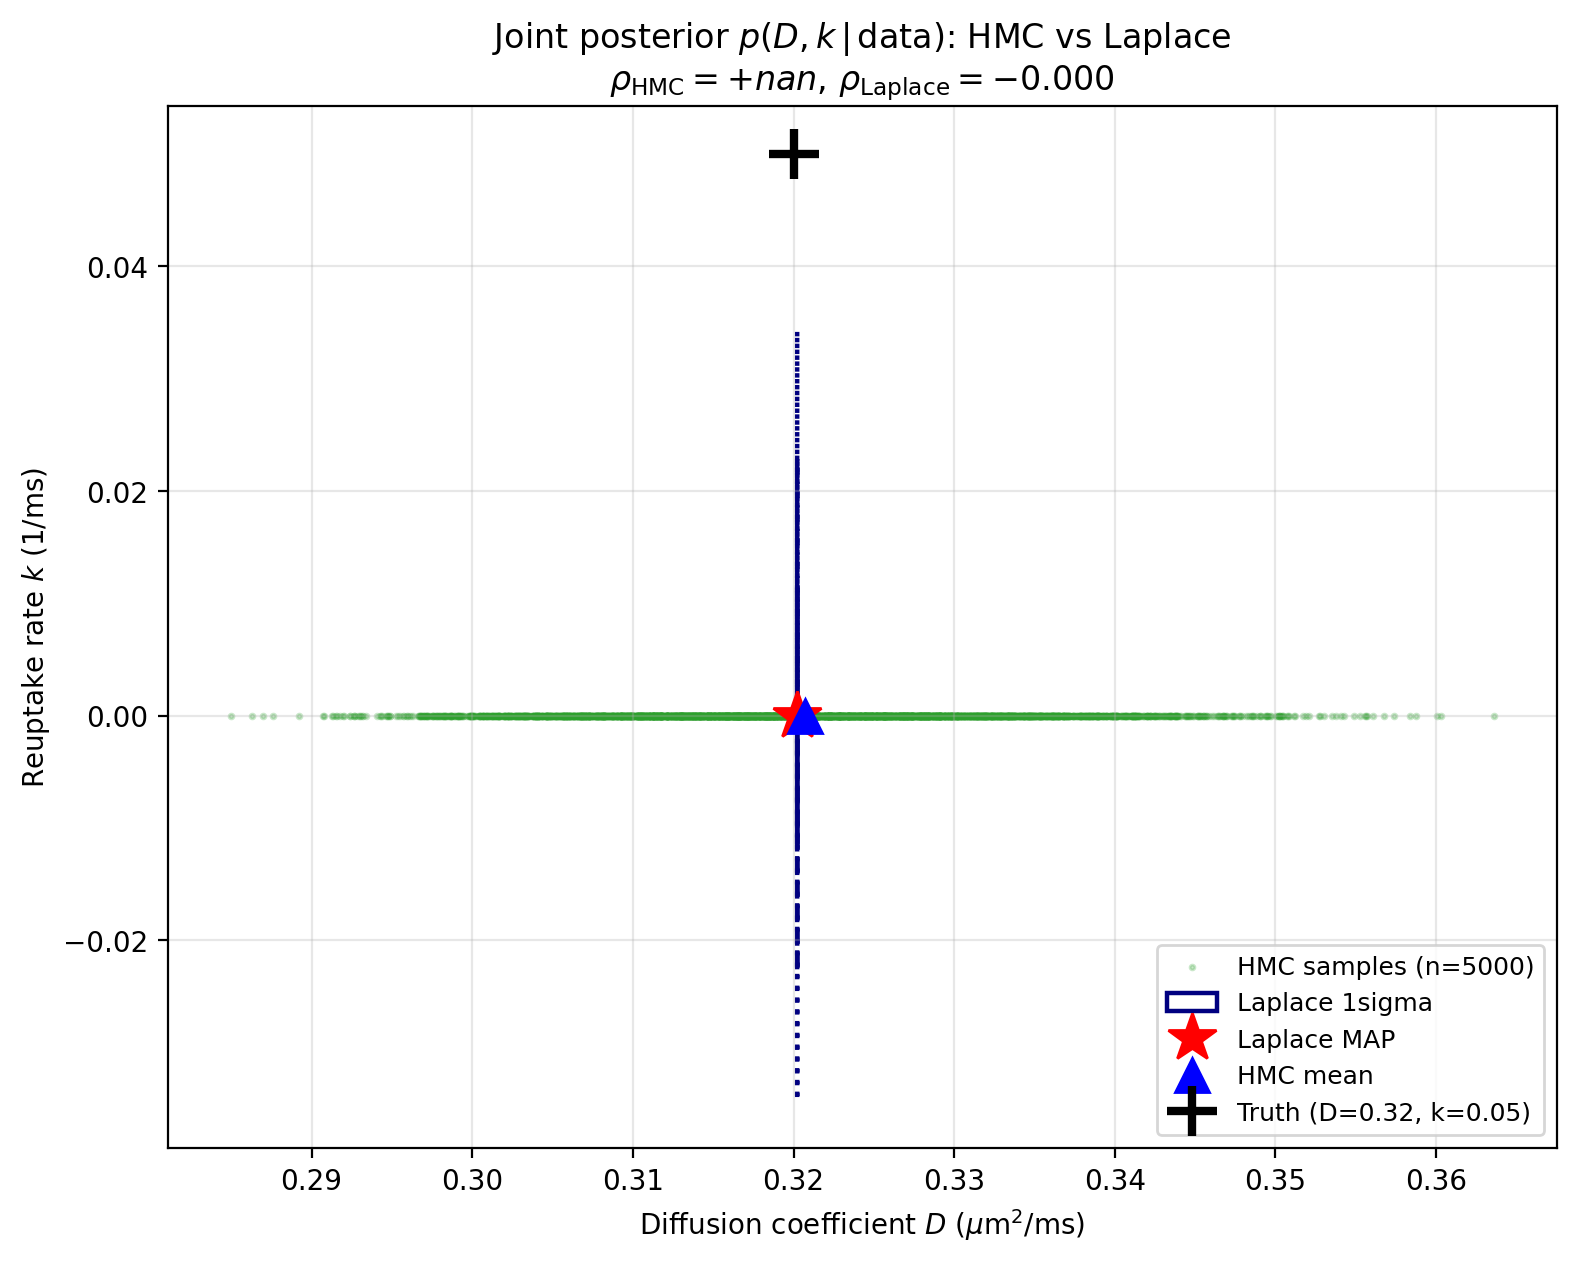
\includegraphics[width=0.9\textwidth]{posterior_hmc.png}
  \caption{\textbf{HMC samples overlaid on Laplace confidence ellipses.}
  Green scatter: $5{,}000$ HMC samples from the analytical-model
  posterior over $(D, k)$. Navy ellipses: Laplace-approximated $1\sigma$
  (solid), $2\sigma$ (dashed), and $3\sigma$ (dotted) confidence regions
  in the $D$ direction. Red star: Laplace MAP. Blue triangle: HMC
  posterior mean. Black plus: ground-truth
  $(D^*, k^*) = (0.32, 0.05)$. The HMC sample cloud and the Laplace
  ellipses agree closely in the $D$ direction, validating the Gaussian
  approximation. Both methods collapse to $k \to 0$ along the
  log-parameter boundary because the infinite-domain analytical model
  cannot fit the elevated late-time concentrations present in the
  bounded-domain observation data.}
  \label{fig:posterior_hmc}
\end{figure}

The two methods agree closely in the $D$ direction: Laplace returns
$D = 0.3202 \pm 0.0114$ and HMC returns $D = 0.3207 \pm 0.0114$,
matching to three decimal places in both posterior mean and standard
deviation. Both $95\%$ credible intervals
($[0.298, 0.343]$ for Laplace and $[0.299, 0.344]$ for HMC) cover the
ground-truth value $D^* = 0.32$. This agreement validates the Gaussian
approximation underlying Laplace for the $D$-dimensional marginal
posterior; the Laplace approximation, which requires only a single
Hessian evaluation, is therefore recommended as the default UQ method
for $D$.

The $k$-dimensional marginal posterior, however, collapses to the
lower boundary of the log-parametrized space ($k \to 0$, corresponding
to $\tilde{k} \to -\infty$) for both methods. This is not a numerical
artifact: it reflects a model-misspecification failure of the
infinite-domain analytical solution when used as the data-likelihood
forward model on bounded-domain observation data. The same failure
appears in the Levenberg--Marquardt baseline reported in the main
text, where the analogous unbounded optimization drives $k$ to a
non-physical negative value ($k_{\mathrm{LM}} = -0.040$). The
structural cause is that bounded-domain dopamine accumulates at late
times due to boundary reflections, producing concentrations higher
than the infinite-domain analytical prediction; the data-likelihood
compensates by reducing $k$ to suppress the analytical model's
exponential decay.

The PINN inverse formulation described in the main text, which uses
the bounded-domain residual loss rather than the analytical model as
the forward map, recovers physically meaningful $k$ values
($k = 0.0573 \pm 0.0006$ across five seeds) and is the recommended
estimator for $k$. A fully consistent Bayesian uncertainty for $k$
would require profile-likelihood retraining of the PINN at each
candidate $(D, k)$ pair, which is computationally expensive and is
identified as a direction for future work.

\end{document}
